\documentclass{beamer}
\mode<presentation>
{
  \usetheme{Rochester}
  % Pittsburgh, Dresden, Boadilla, Berlin, Goettingen, Luebeck, Rochester
  \setbeamercovered{transparent}
}

\usepackage[german]{babel}
\usepackage[latin1]{inputenc}
\usepackage[T1]{fontenc}
\usepackage{eurosym}
\usepackage{lmodern}
%\usepackage{times}

\title[Bericht 2. PSS]{2. PSS bei der Seitenbau GmbH}
\author[J.~Tammen]{Jan Tammen, SE 7}

\institute{
  Fakult�t Informatik,\\
  Studiengang Software-Engineering,\\
  HTWG Konstanz
}

%%% Informationen ueber das PDF-Dokument setzen
\hypersetup{
  pdftitle={2. PSS bei der Seitenbau GmbH},%
  pdfauthor={Jan Tammen},%
  pdfsubject={Praxissemesterbericht},%
  pdfcreator={LaTeX with pdfeTeX},%
  pdfproducer={LaTeX with pdfeTeX},%
  % pdfpagelayout=TwoColumnRight,
  pdffitwindow=true,
  pdfpagemode=FullScreen,
%  pdfstartview=FitH,
}

\date{13.\,Dezember 2006}
\subject{Praxissemesterbericht 2. PSS}

\pgfdeclareimage[height=1cm]{htwg-logo}{../images/htwg-logo}
\logo{\pgfuseimage{htwg-logo}}

% Folgendes sollte gel�scht werden, wenn man nicht am Anfang jedes
% Unterabschnitts die Gliederung nochmal sehen m�chte.
% \AtBeginSubsection[]
% {
%  \begin{frame}<beamer>
%    \frametitle{Gliederung}
%    \tableofcontents[currentsection,currentsubsection]
%  \end{frame}
% }

% Falls Aufz�hlungen immer schrittweise gezeigt werden sollen, kann
% folgendes Kommando benutzt werden:
\beamerdefaultoverlayspecification{<+->}

\begin{document}

% Frame: Titelseite
\begin{frame}
  \titlepage
\end{frame}

% Frame: Anzeige der Gliederung / Inhaltsverzeichnis
\begin{frame}
  \frametitle{Gliederung}
  \tableofcontents
  % Die Option [pausesections] k�nnte n�tzlich sein.
\end{frame}

\section{SEITENBAU GmbH}
\subsection{Allgemeines}

% Frame: Vorstellung der Firma
\begin{frame}
  \frametitle{Die SEITENBAU GmbH}
  
  \begin{itemize}
    \item Internet-Full-Service-Agentur
    \item Hauptsitz in Konstanz
    \item bietet zahlreiche Dienstleistungen im Bereich Web- und
    Softwareentwicklung an
  \end{itemize}
\end{frame}

\subsection{Dienstleistungen und Produkte}
\begin{frame}
  \frametitle{Dienstleistungen und Produkte}
  
  \begin{itemize}
    \item CMS - Content Management Systeme
    \item Webentwicklung: Beratung, Konzeption u. Realisierung; Barrierefreiheit
    \item \url{www.bonn.de}, \url{www.konstanz.de},
    \url{www.illbruck-online.de}, \ldots
    \item Softwareentwicklung, z.\,B.\ in Java (Bundesverwaltungsamt, T-Online)
  \end{itemize}
\end{frame}

\subsection{Zahlen und Fakten}
\begin{frame}
  \frametitle{Zahlen und Fakten}
  
  \begin{itemize}
    \item gegr�ndet 1996
    \item derzeit 41 feste Mitarbeiter
    \item Hauptsitz in Konstanz, Niederlassung in K�ln
    \item Umsatz 2005: ca.\ 2,45 Mio.\ \euro
  \end{itemize}
\end{frame}

\section{Projekte und Aufgaben}
\subsection{Allgemeine Aufgaben}
\begin{frame}
  \frametitle{Projekte und Aufgaben}
  \frametitle{Allgemeine Aufgaben}
  
  \begin{itemize}
    \item PHP, Perl, Java
    \item relationale Datenbanken, SQL
    \item JavaScript, XHTML
    \item XML/XSL-T, AJAX
  \end{itemize}
\end{frame}

\subsection{Projekte}
\begin{frame}
  \frametitle{Projekte}
  \framesubtitle{PHP-Framework}
  
  \begin{block}{Aufgabenstellung}
    Erstellung eines Frameworks f�r "`CRUD"'-Anwendungen.
  \end{block}
  
  \begin{block}{Ablauf}
    \begin{enumerate}
      \item Design und Entwurf (OOA/OOD mit UML), Verwendung des (abgewandelten)
      MVC-Paradigmas
      \item Implementierung (Umsetzung mittels PHP\,4)
      \item Portierung bestehender Anwendungen, kleinere Anpassungen
    \end{enumerate}
  \end{block}
\end{frame}

\begin{frame}
  \frametitle{PHP-Framework}
  \frametitle{UML-Klassendiagramm (Analysephase)}
  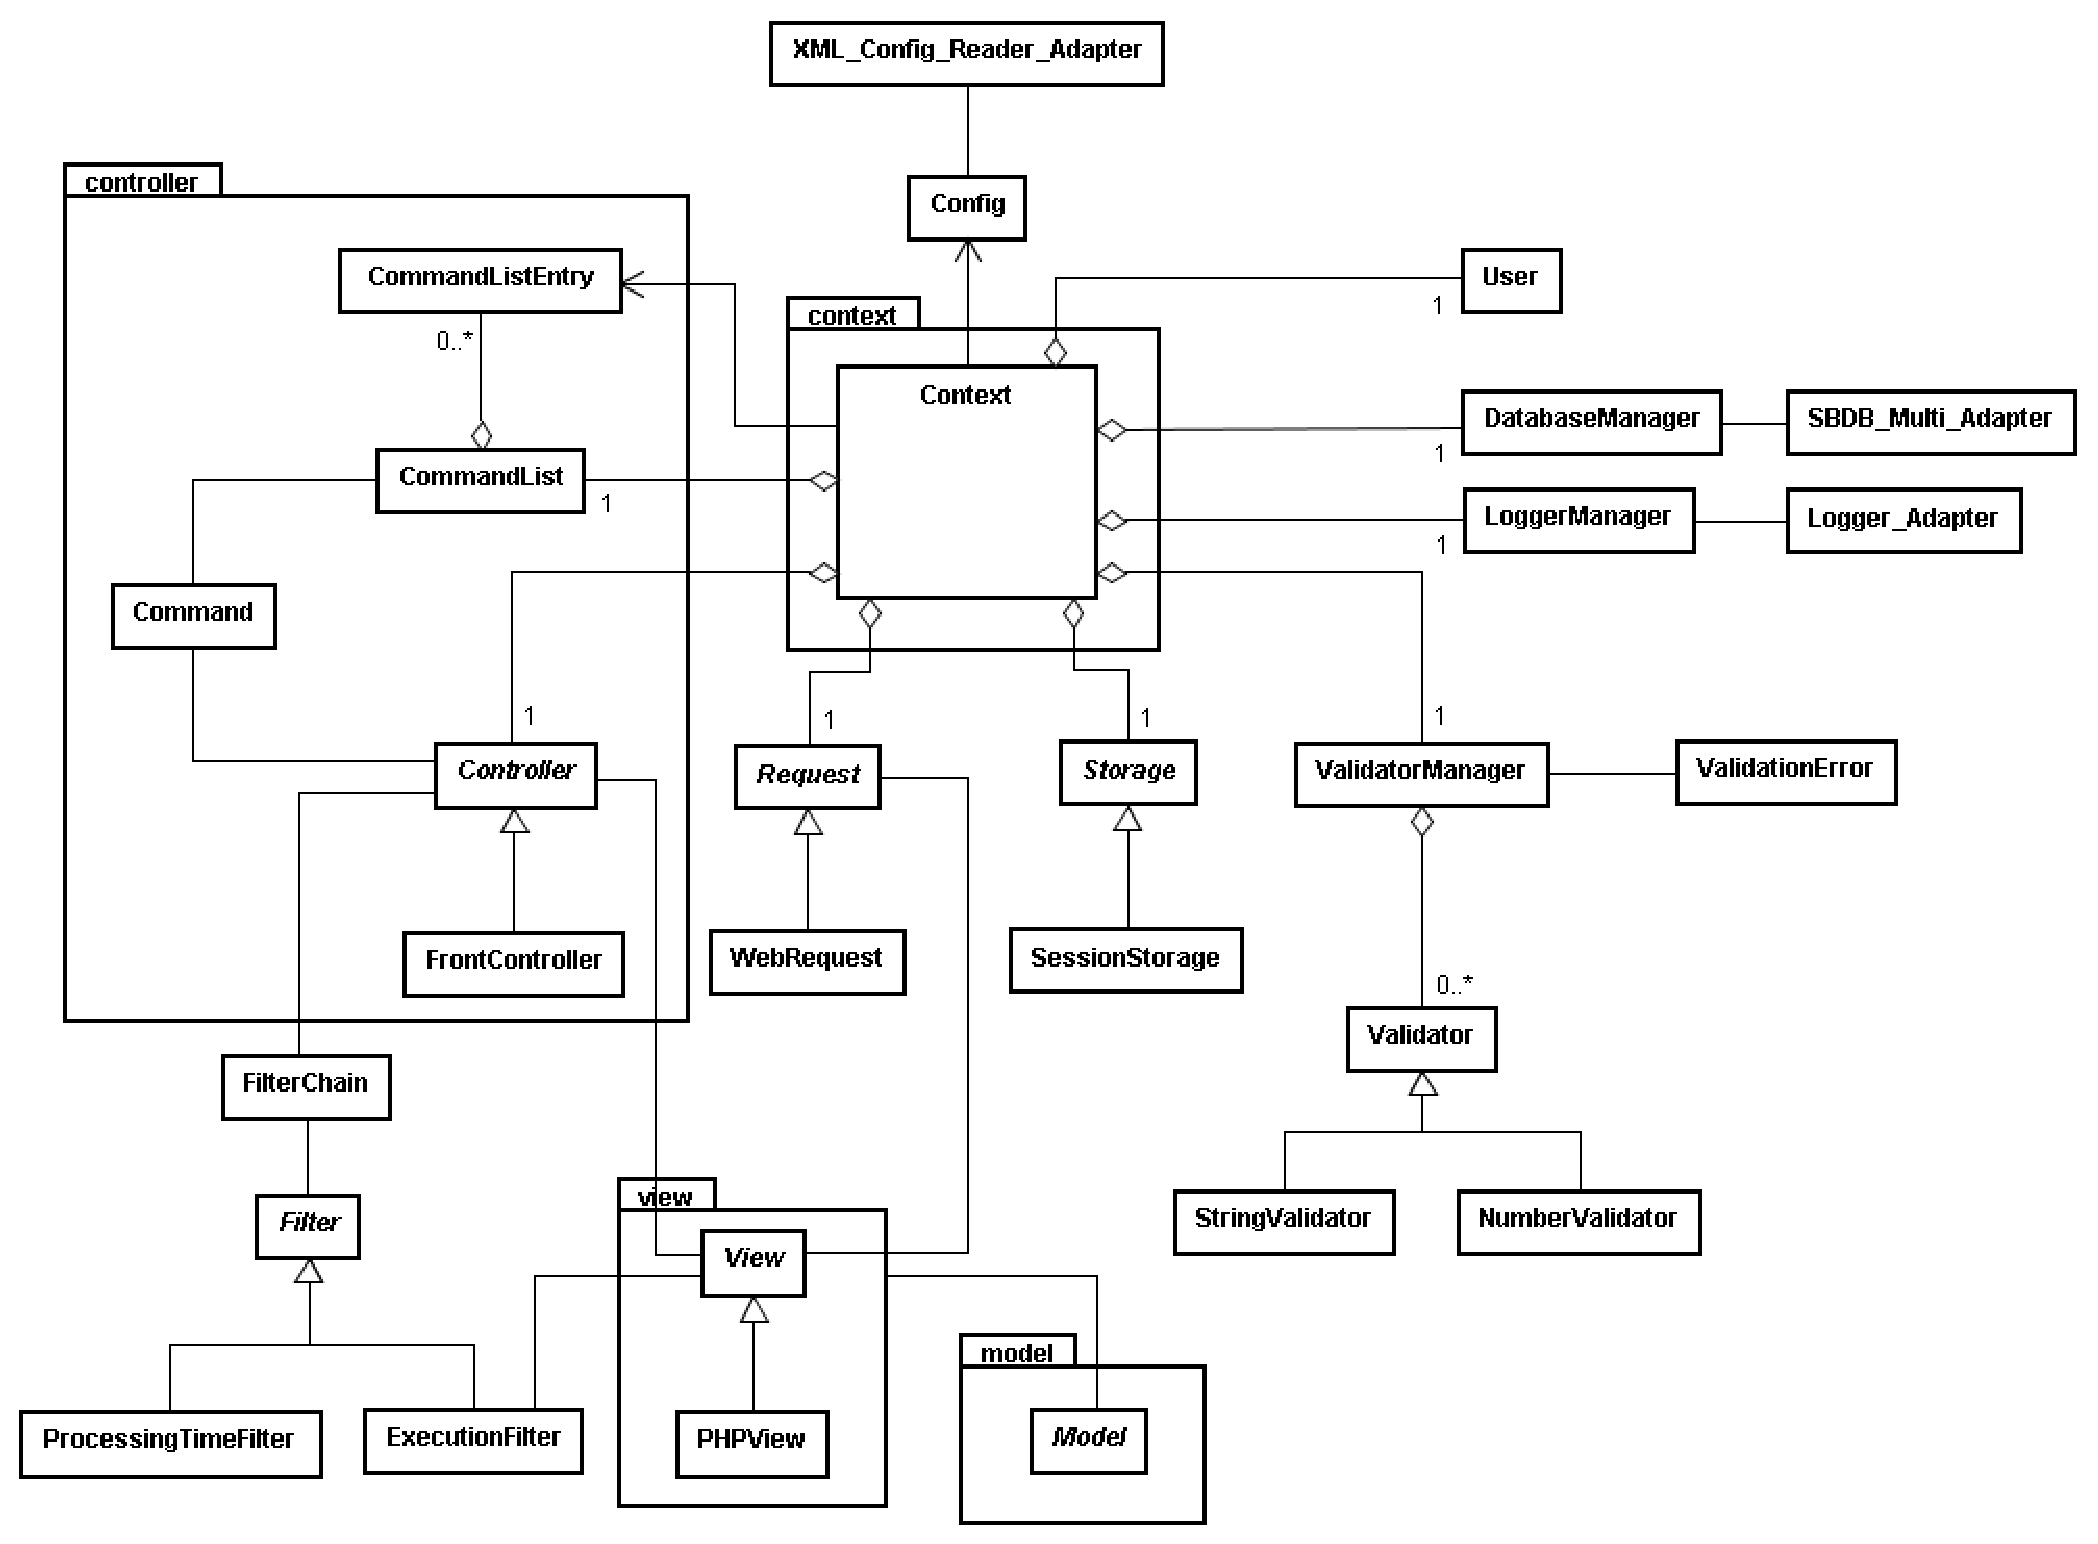
\includegraphics[width=0.90\textwidth]{../images/framework-klassendiagramm}
\end{frame}

\begin{frame}
  \frametitle{Projekte}
  \framesubtitle{LAUT Klublandschaft}
  
  \begin{block}{Aufgabenstellung}
    Visualisierung von Veranstaltungsterminen auf einer Karte, hier mit der
    Google-Maps-API ("`Mashup"').
  \end{block}
  
  \begin{block}{Ablauf}
    \begin{enumerate}
      \item Einarbeitung in die obj.orient. JavaScript-API von Google
      \item Implementierung der Serverseite, AJAX-Ansatz
      \item Implementierung der Clientseite, JavaScript f�r Verwaltung der
      Marker etc.
      \item Implementierung der GUI, teilw. statisches XHTML, Rest via
      clientseitiger XSL-Transformationen
    \end{enumerate}
  \end{block}
\end{frame}

\begin{frame}
  \frametitle{LAUT Klublandschaft}
  \frametitle{�bersicht}
  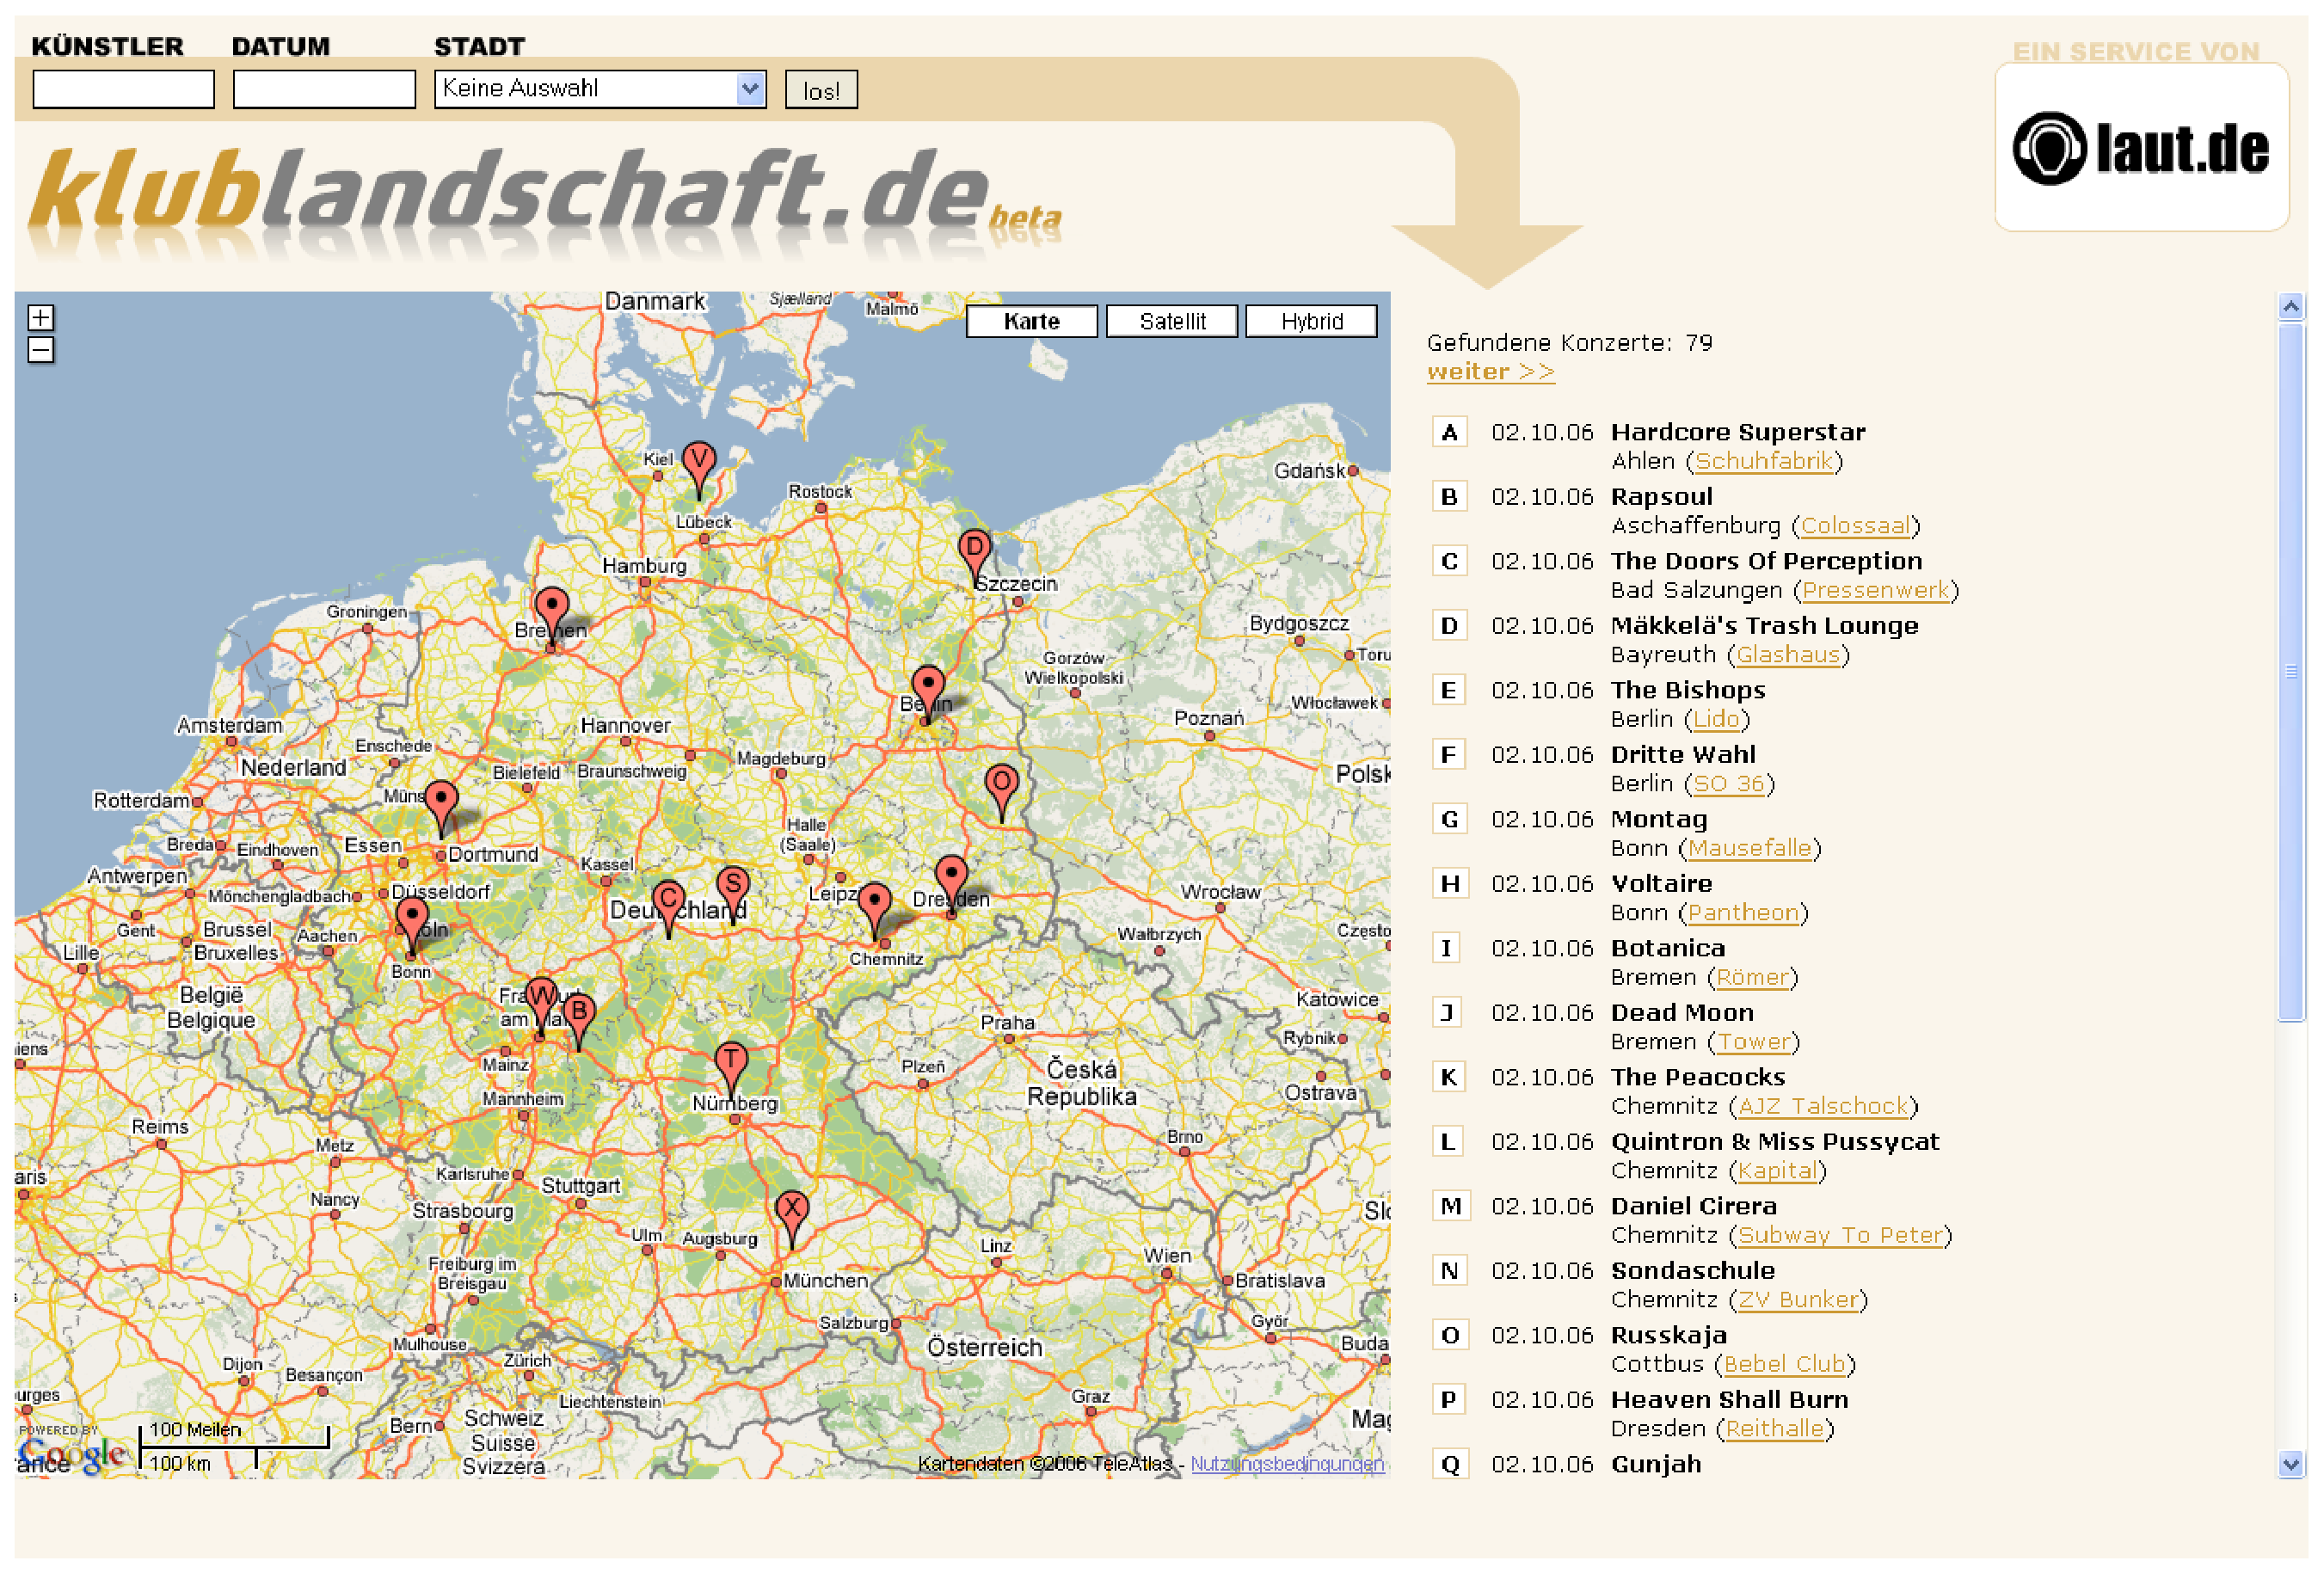
\includegraphics[width=1.00\textwidth]{../images/klublandschaft-uebersicht}
\end{frame}

\begin{frame}
  \frametitle{LAUT Klublandschaft}
  \frametitle{Infofenster eines Markers}
  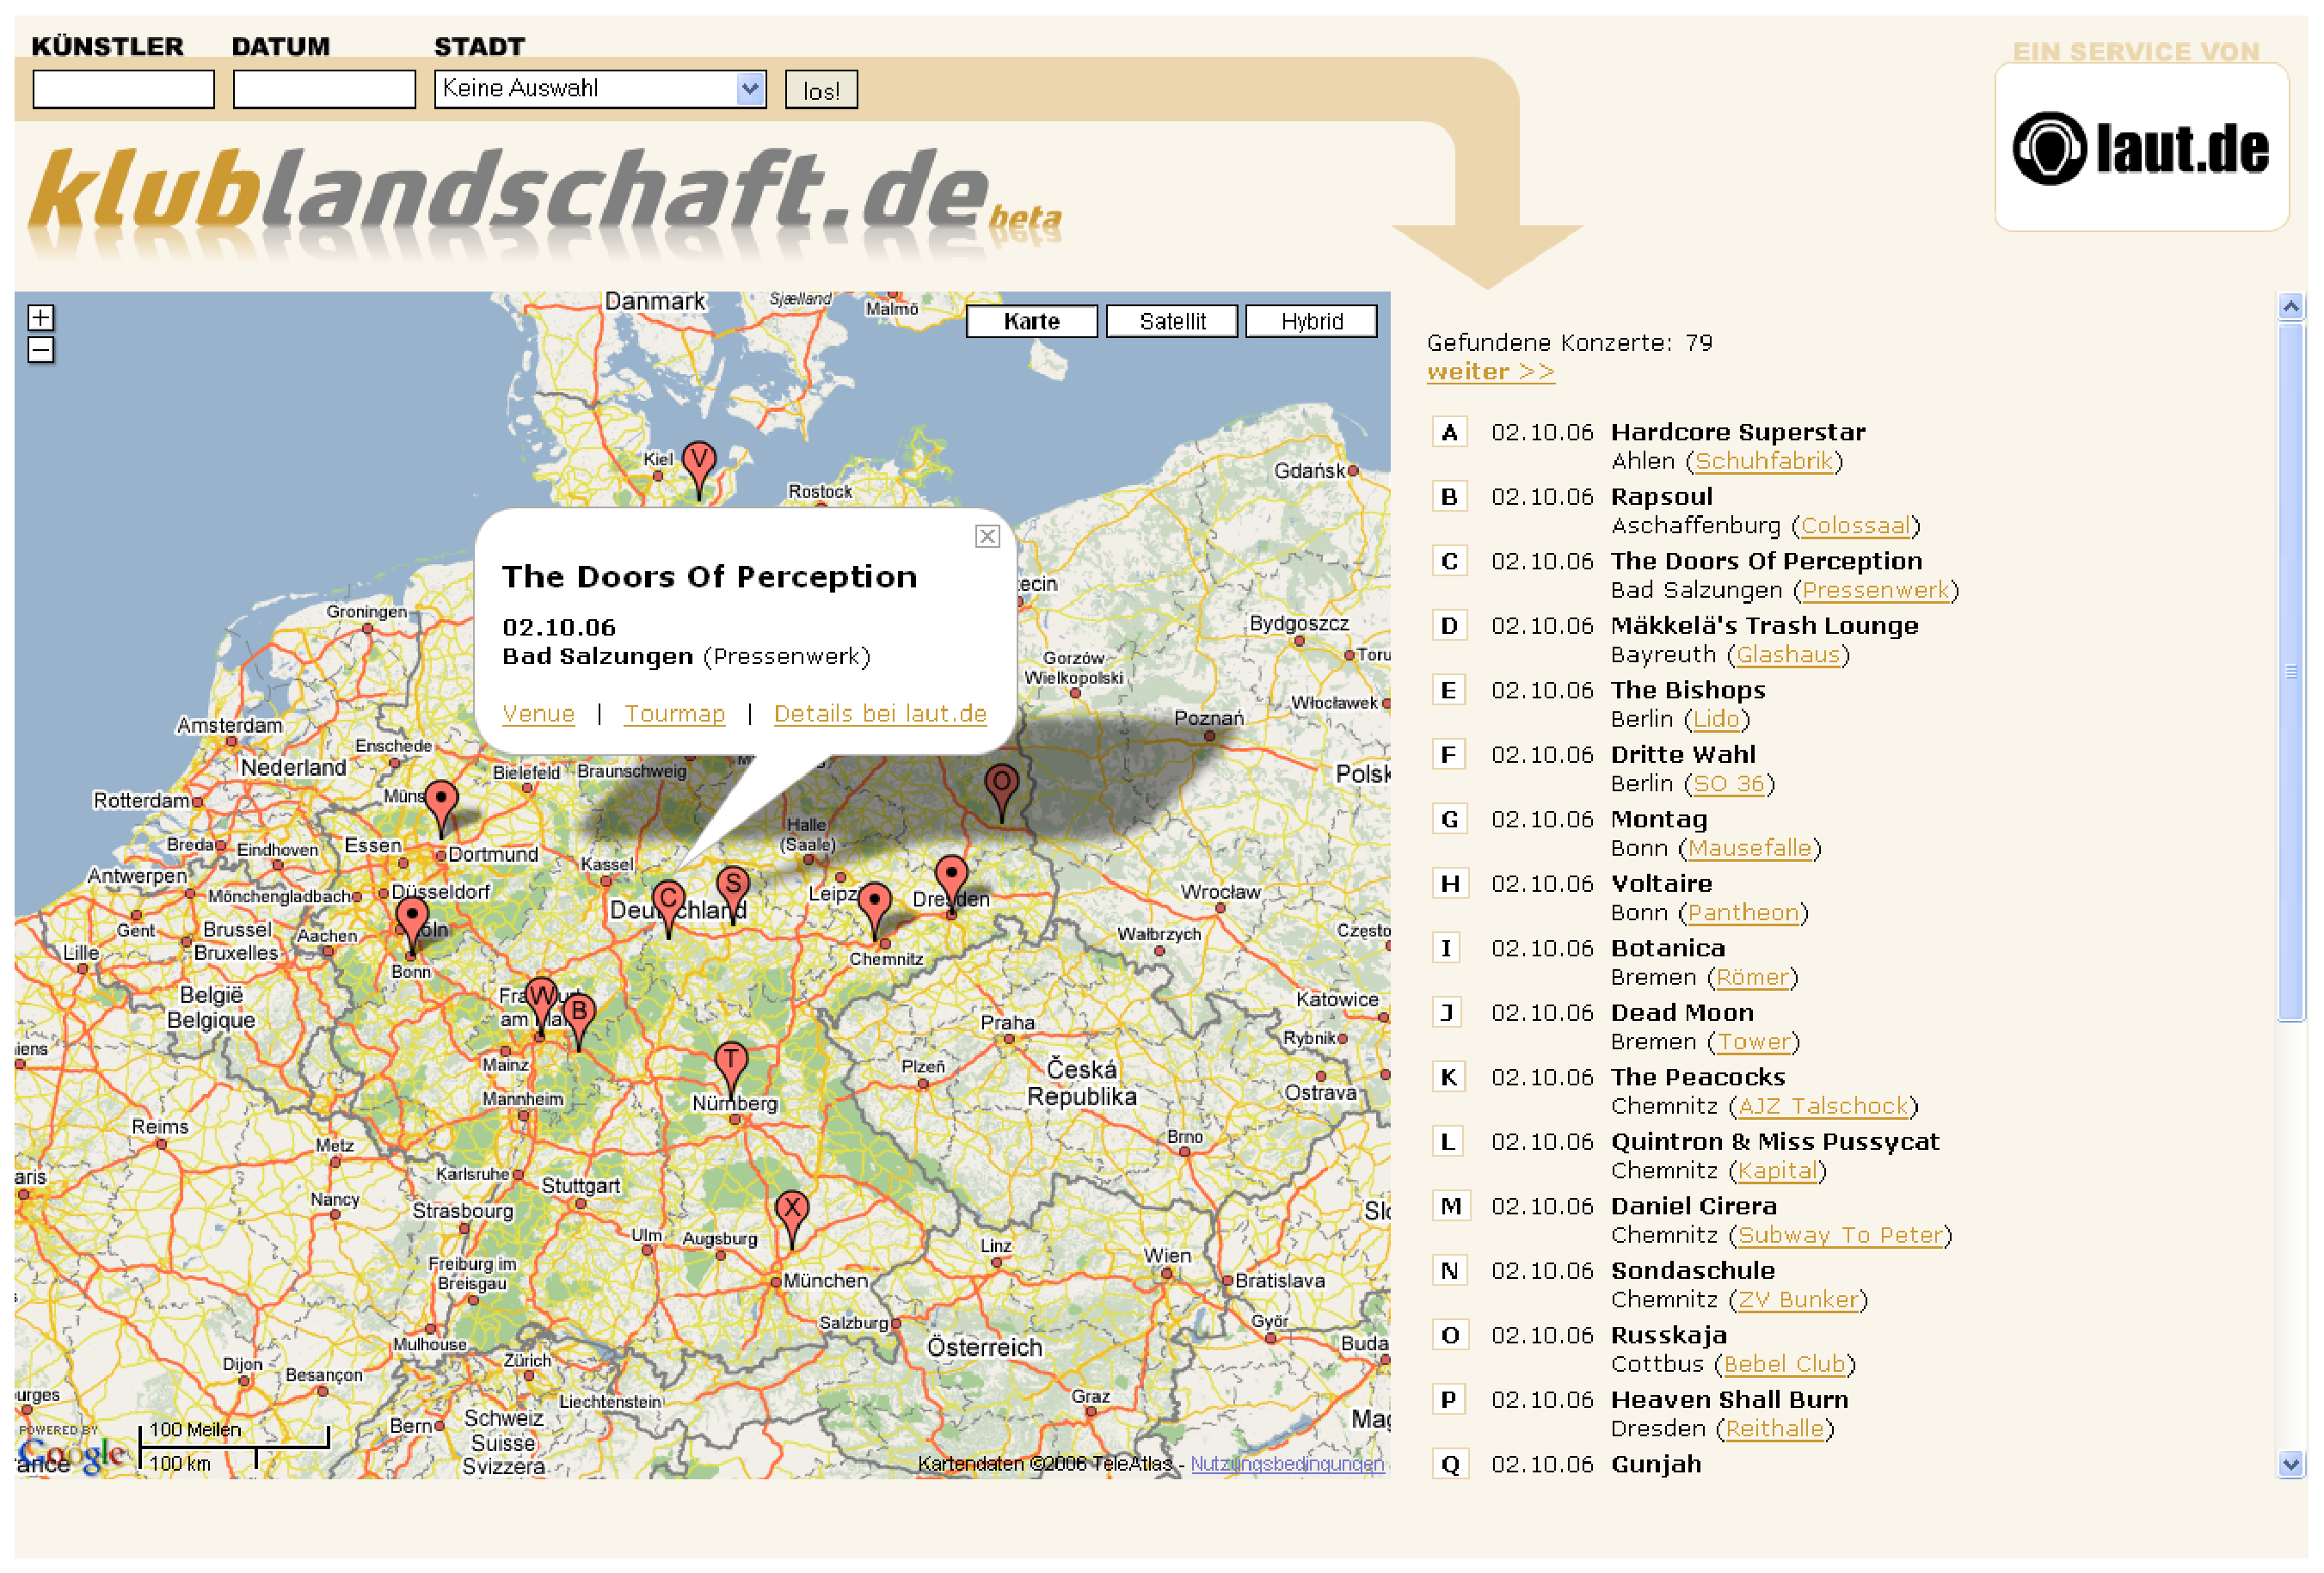
\includegraphics[width=1.00\textwidth]{../images/klublandschaft-uebersicht-infowindow}
\end{frame}

\begin{frame}
  \frametitle{LAUT Klublandschaft}
  \frametitle{Detailansicht einer Veranstaltung}
  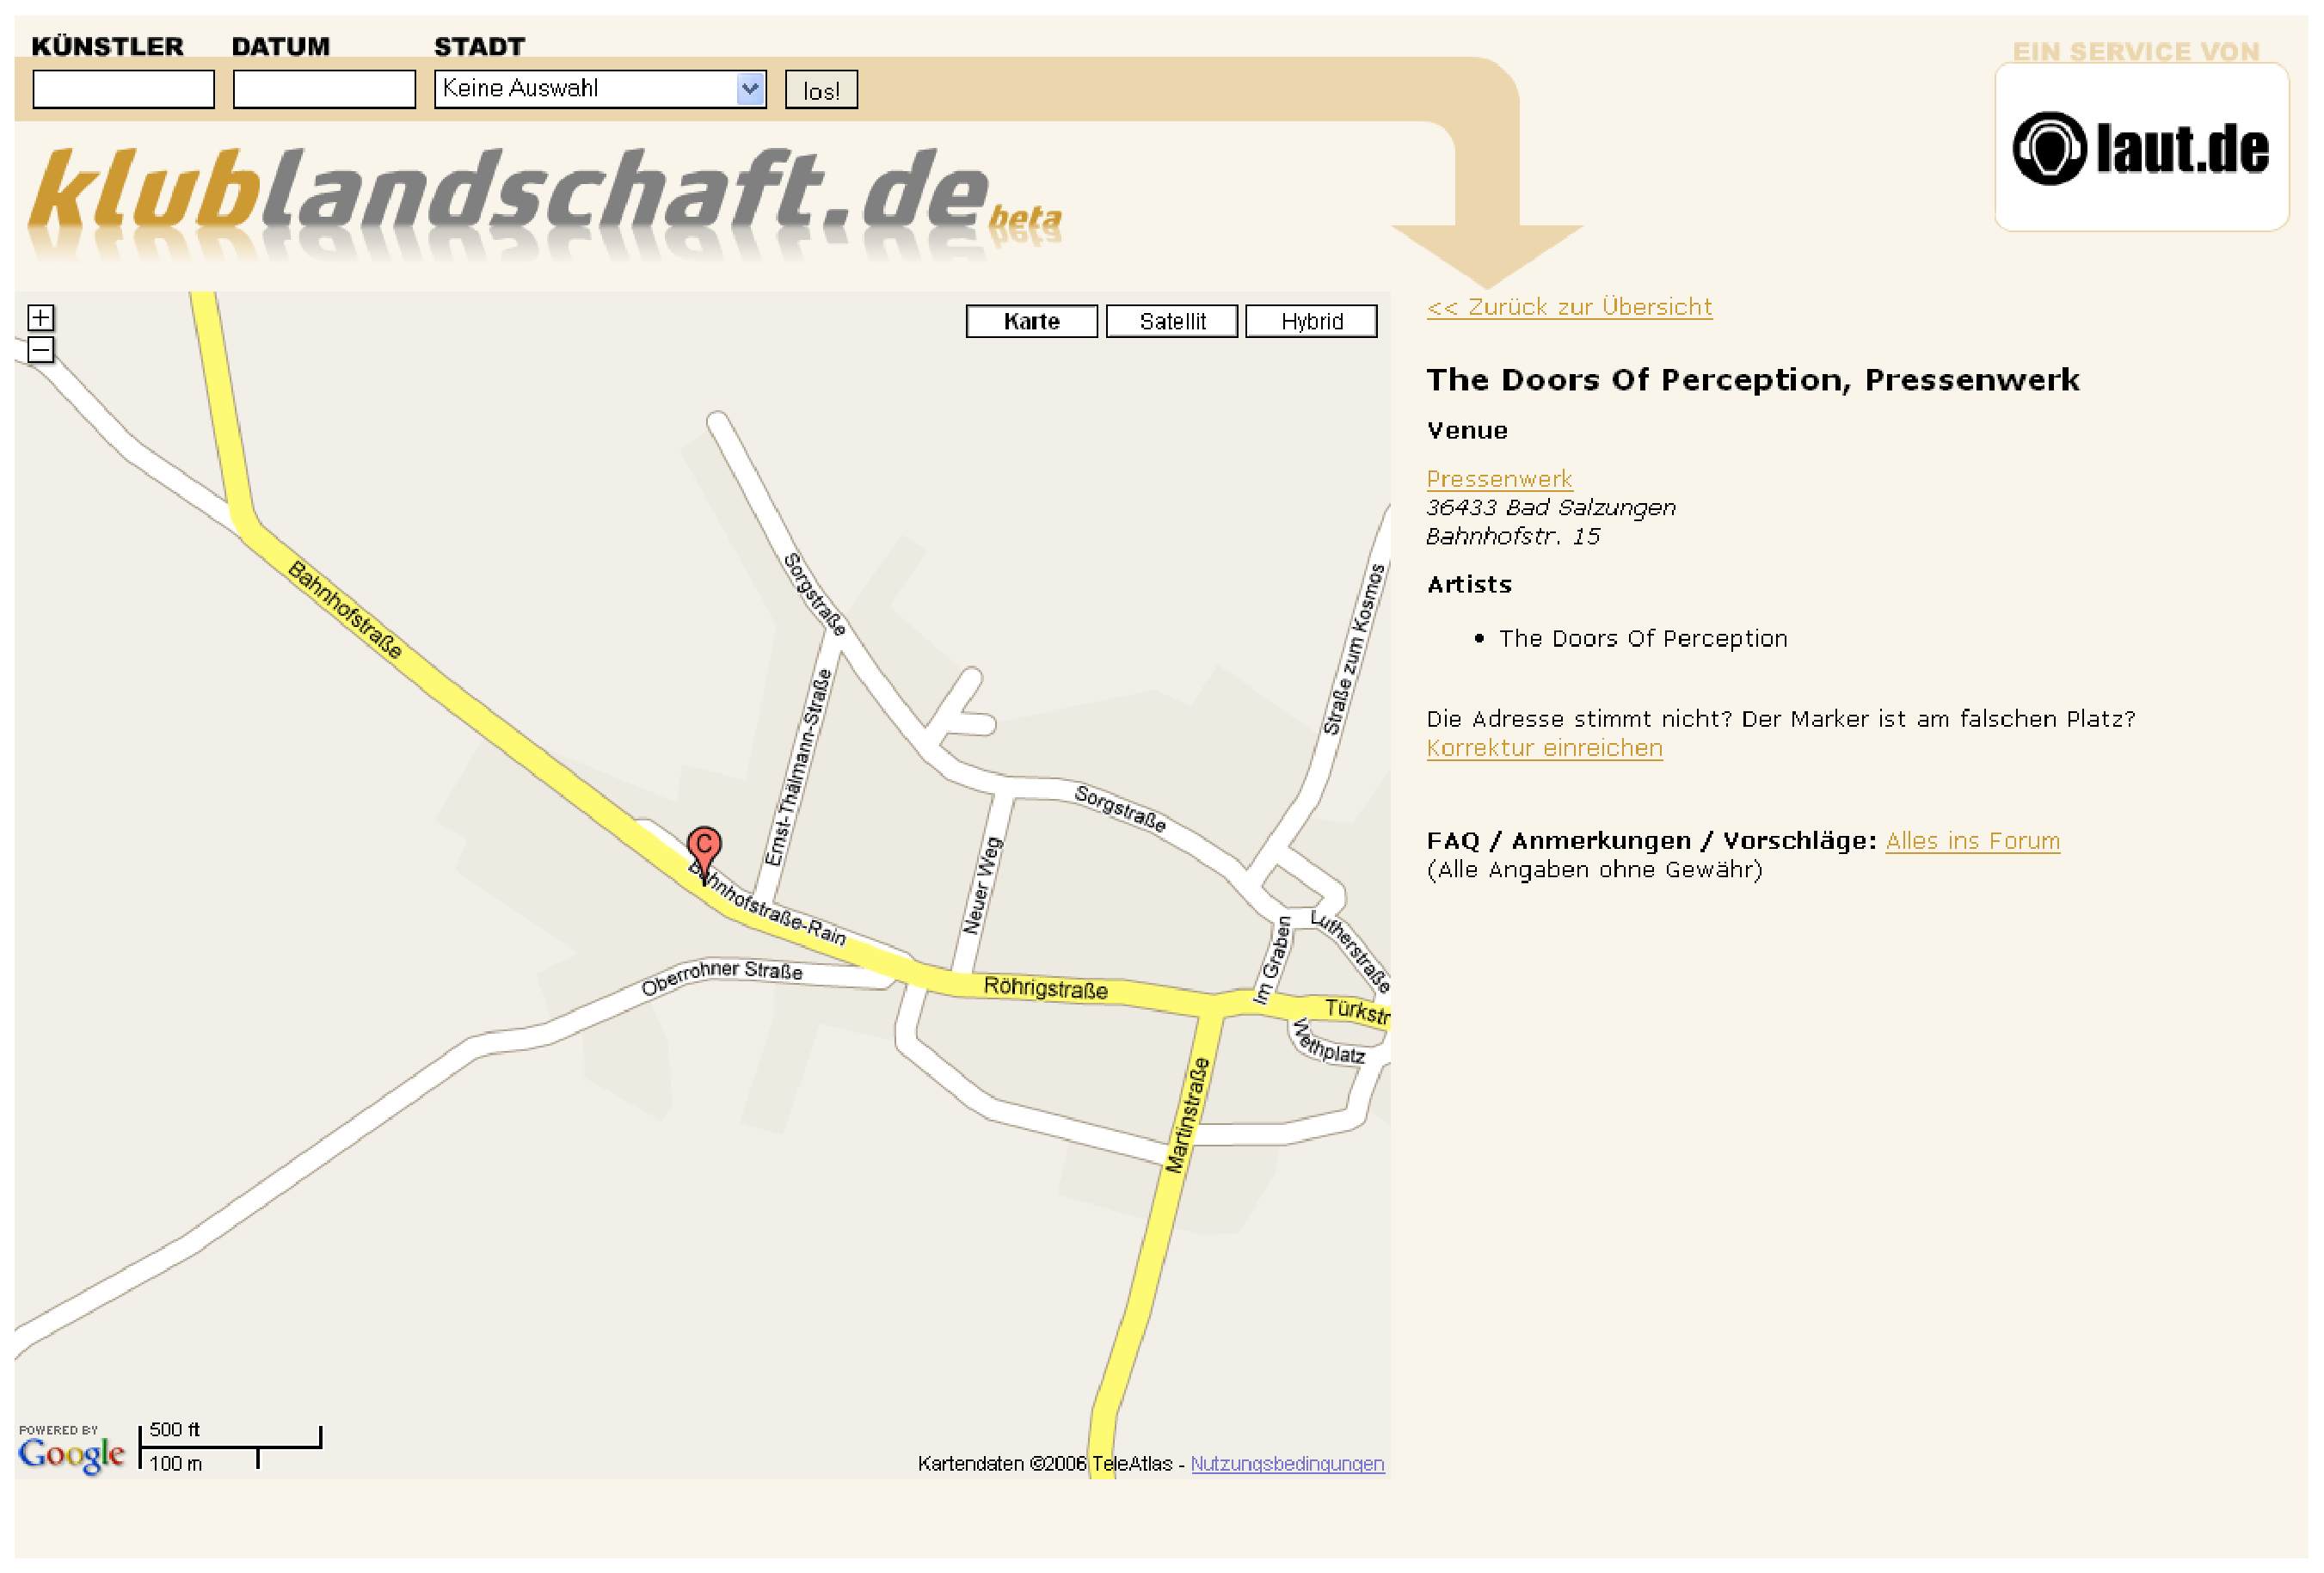
\includegraphics[width=1.00\textwidth]{../images/klublandschaft-venue}
\end{frame}

\section{Soziales Umfeld und Fazit}
\begin{frame}
  \frametitle{Soziales Umfeld}
  
  \begin{itemize}
    \item Gleitzeit, 40h-Woche, freie Pauseneinteilung
    \item nette, hilfsbereite Kollegen und Kolleginnen
    \item insgesamt recht junges Team, lockerer Umgangston ("`Du"')
  \end{itemize}
\end{frame}

\begin{frame}
  \frametitle{Mein Fazit}
  
  \begin{itemize}
    \item sowohl fachliche als auch soziale Erkenntnisse gewonnen
    \item in interessanten und anspruchsvollen Projekten
    \item sehr angenehmes Arbeitsumfeld
  \end{itemize}
  
  \pause
  
  \centering
  $\Rightarrow$ empfehlenswerter Praktikumsplatz!
  
\end{frame}

\begin{frame}
  \frametitle{Danke.}
  Noch Fragen?
\end{frame}

\end{document}